\section{Análise e Justificativa do Projeto}

As escolhas do sistema embarcado do Logan foram definidas a partir da convergência entre os requisitos do regulamento da EletroQuad SAE Brasil 2026, as demandas operacionais das missões previstas e os aprendizados acumulados pela equipe no ciclo anterior. Dessa forma, a seleção dos componentes não foi tratada apenas como uma etapa de montagem, mas como uma decisão de engenharia orientada por critérios de compatibilidade, confiabilidade, consumo energético, integração entre módulos e viabilidade de operação em competição.

Além do atendimento aos componentes obrigatórios e às restrições impostas pelo regulamento, buscou-se priorizar soluções com boa maturidade de uso, disponibilidade no mercado nacional, documentação consolidada e integração já validada com o restante da arquitetura do drone. Também foram considerados fatores como massa embarcada, facilidade de manutenção, estabilidade elétrica, robustez frente a vibrações e interferências, além da capacidade do sistema de sustentar as três missões da competição sem exigir alterações profundas entre configurações.

\subsection{Critérios de seleção}

A seleção dos componentes do Logan foi guiada por cinco critérios principais: conformidade com o regulamento, compatibilidade entre subsistemas, adequação às missões, eficiência energética e confiabilidade operacional. Esses critérios foram adotados porque a competição impõe restrições explícitas quanto à configuração da aeronave, aos sensores permitidos, ao firmware da controladora, à presença obrigatória de telemetria e ao monitoramento elétrico da bateria.

Do ponto de vista funcional, os componentes escolhidos precisavam permitir controle estável da aeronave, comunicação entre a controladora e o computador de bordo, aquisição confiável de dados sensoriais e suporte às tarefas de percepção visual exigidas nas missões. Ao mesmo tempo, a seleção também precisou respeitar critérios não funcionais, como limitação de peso, simplicidade de integração, facilidade de substituição e redução de vulnerabilidades observadas em 2025.

Outro critério importante foi a maturidade técnica das soluções adotadas. Em vez de priorizar componentes mais sofisticados apenas pelo apelo tecnológico, optou-se por itens amplamente documentados, já utilizados pela equipe ou consolidados na comunidade de drones com ArduPilot, reduzindo risco de integração e acelerando o processo de validação.

\subsection{Justificativa por módulo}

A justificativa das escolhas foi organizada segundo a mesma divisão funcional apresentada na arquitetura do sistema embarcado. Essa correspondência entre as seções passada e a atual foi adotada para manter coerência estrutural no relatório: enquanto a seção passada descreve como o sistema está dividido e conectado, esta subseção discute por que cada módulo foi configurado da forma escolhida. Dentro de cada módulo, os componentes são analisados em termos de função, critério de seleção, vantagem prática e aderência às restrições da competição.

\subsubsection{Módulo de propulsão}

\paragraph{Motores:}
Os motores brushless Turnigy D2386/8 de 1100kV foram mantidos como referência no Logan pelo bom histórico de uso no projeto e integração já validada com o resto do seu módulo (ESCs e bateria). Sua seleção foi favorecida pela capacidade de fornecer empuxo suficiente ao envelope de voo pretendido, sem impor aumento excessivo de massa ou demanda elétrica desproporcional ao restante do sistema. Além disso, a equipe adquiriu seis motores Angel D2368 de 1120kV para realização de ensaios comparativos em bancada. Os testes indicaram desempenho de empuxo bastante próximo ao observado nos motores Turnigy, sem diferença prática suficientemente expressiva para justificar a exclusão imediata de uma das opções. Dessa forma, o projeto passou a considerar dois conjuntos de motorização viáveis para o Logan: quatro motores Angel ou quatro motores Turnigy, sempre utilizando um único modelo (quatro motores da mesma marca) por montagem. Em razão dessa equivalência observada nos testes e da possibilidade real de uso de qualquer um dos dois conjuntos, ambas as opções estão registradas neste relatório.

\paragraph{ESCs:}
Os ESCs Hobbywing Skywalker 40A V2 foram selecionados por oferecerem corrente nominal compatível com o conjunto motopropulsor adotado, além de ampla utilização em aplicações de aeromodelismo e multirrotores. A adoção destes ESCs com uma margem de corrente razoável também contribui para reduzir estresse elétrico nos acionamentos e elevar a confiabilidade do módulo de propulsão. Assim, a escolha desse componente não se deu apenas por disponibilidade, mas pelo equilíbrio entre custo, resposta dinâmica e margem de segurança válida.

\subsubsection{Módulo de alimentação}

\paragraph{Bateria:}
A bateria LiPo Turnigy Rapid 4S2P de 8000mAh e 140C foi escolhida por oferecer não apenas maior capacidade energética, mas principalmente melhor comportamento elétrico sob carga quando comparada à bateria anteriormente utilizada. A substituição foi motivada pelos problemas observados com a bateria Teranty 4S de 6500mAh, que apresentava queda acentuada de tensão em demandas elevadas de corrente, comprometendo o tempo de voo e acionando prematuramente mecanismos de \textit{failsafe} da controladora.

Do ponto de vista construtivo, a arquitetura eletroquímica 4S2P (quatro células em série, 2 células em paralelo) reduz a resistência interna equivalente do pacote em relação à arquitetura 4S (quatro células em série), o que contribui para mitigar o \textit{voltage sag} durante acelerações e variações bruscas de carga. Com isso, a tensão terminal se mantém mais estável durante a operação, favorecendo tanto o sistema de propulsão quanto a alimentação dos módulos eletrônicos embarcados.

Além disso, a bateria adotada mantém compatibilidade com a arquitetura elétrica do Logan, fornece margem mais confortável para picos de corrente e amplia a disponibilidade energética útil do sistema sem impor uma penalização excessiva de massa para a aeronave. Assim, sua escolha foi guiada por autonomia, estabilidade elétrica e confiabilidade operacional, e não apenas por aumento nominal de capacidade. 

\paragraph{Placa de distribuição de energia:}
A utilização da PDB Matek XT60 foi priorizada por centralizar a distribuição de potência em um único ponto, simplificando o roteamento elétrico entre bateria, ESCs e demais módulos. Esse arranjo favorece organização interna, reduz emendas desnecessárias e melhora a rastreabilidade das conexões, o que é especialmente importante em atividades de manutenção, inspeção e diagnóstico de falhas. A centralização da distribuição também contribui para maior clareza no projeto elétrico da aeronave. Em sistemas embarcados de pequeno porte, uma arquitetura energética organizada reduz risco de erro humano na montagem e facilita intervenções ocasionais sem necessidade de reconfiguração extensa do cabeamento.

\paragraph{Regulador de tensão e power module:}
O uso conjunto do Power Module e do regulador de tensão MH-KC24 foi adotado para separar adequadamente a alimentação da controladora de voo e do computador de bordo. Essa decisão decorre das características distintas desses dois tipos de carga: enquanto a Pixhawk exige alimentação estável e monitorada para execução do controle de voo, a Raspberry Pi 5 demanda uma linha de alimentação mais robusta e com maior margem de corrente, compatível com seu perfil computacional. A própria fonte oficial da Raspberry Pi 5 fornece 5,1V a até 5A como perfil principal, além de perfis \textit{Power Delivery} adicionais de 9V @ 3A, 12V @ 2,25A e 15V @ 1,8A. 

Nos testes iniciais, verificou-se que a alimentação constante em 5V aplicada à Raspberry Pi permitia o acionamento e o processo de boot, mas ainda resultava em registros de subtensão (\textit{brownout}) e, posteriormente, em desligamentos recorrentes do sistema. Diante desse comportamento, foi implementado um regulador dedicado com suporte a \textit{Power Delivery}, o MH-KC24, buscando fornecer ao computador de bordo uma alimentação com melhor estabilidade sob carga e maior compatibilidade com suas exigências energéticas.

\begin{figure}[H]
    \centering
    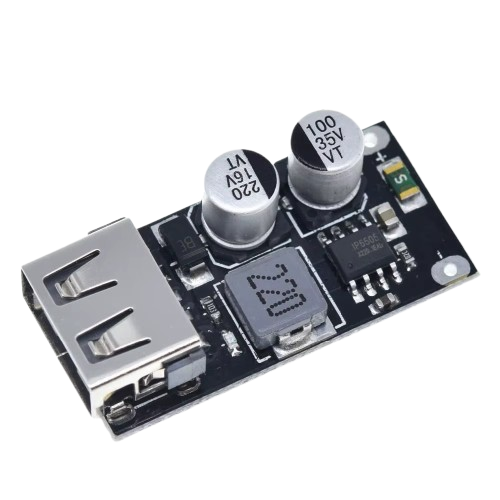
\includegraphics[width=0.5\textwidth]{imagens/mhkc24.png}
    \caption{Regulador de tensão MH-KC24}
    \label{fig:vreg}  
\end{figure}

A escolha do MH-KC24 foi favorecida por sua faixa de entrada de 6V a 32V, potência de até 24W, capacidade de fornecimento de até 5V/3,4A, eficiência declarada entre 90\% e 97\% e proteções contra sobretensão, subtensão, sobrecorrente, curto-circuito e sobretemperatura. Em paralelo, o Power Module foi mantido como elemento dedicado à alimentação e ao monitoramento elétrico da Pixhawk, fornecendo uma linha regulada próxima de 5V e permitindo a medição de tensão e corrente da bateria.

\subsubsection{Módulo de navegação}

\paragraph{Controladora de voo:}
Para 2026, optou-se pela substituição da Pixhawk 2.4.8 pela Pixhawk 6C Pro. A principal motivação foi buscar uma controladora com sensores embarcados mais modernos e maior confiabilidade para as etapas de navegação e estimação de estado, especialmente considerando os problemas enfrentados pela equipe no ciclo anterior.

Além da compatibilidade com o ArduPilot, a Pixhawk 6C Pro oferece IMUs redundantes, aquecimento dos sensores e isolamento de vibração integrado, características que ajudam a reduzir ruído nas medições e tornam a plataforma mais adequada para integração no Logan. Embora isso não elimine erros de configuração ou de montagem, a mudança representa um avanço importante na qualidade da base inercial utilizada pela aeronave.

\paragraph{Firmware:}
A adoção do ArduPilot decorre de sua compatibilidade direta com a Pixhawk 6C Pro, de sua ampla utilização em plataformas de voo autônomo e da boa disponibilidade de documentação técnica. A escolha também foi favorecida pela integração com o Mission Planner, que facilita a configuração, calibração, análise de logs e ajuste de parâmetros ao longo do desenvolvimento. Além disso, o ArduPilot utiliza o protocolo MAVLink, um protocolo leve de comunicação amplamente empregado no ecossistema de drones, o que favorece a troca de dados entre a controladora, a estação de solo e o computador de bordo.

\paragraph{Computador de bordo:}
A Raspberry Pi 5 foi selecionada como computador de bordo por oferecer capacidade computacional compatível com as tarefas de percepção visual, processamento de imagens e execução da lógica embarcada de missão, funções que extrapolam o escopo de atuação da controladora de voo. No Logan, ela complementa a arquitetura com uma camada dedicada ao processamento de alto nível, demarcando assim uma clara separação entre controle crítico e computação não crítica.

Sua escolha também foi favorecida pela compatibilidade direta com o ecossistema de desenvolvimento adotado pela equipe, baseado em Python, OpenCV e integração com os fluxos de navegação e decisão em tempo real. Essa combinação torna a Raspberry Pi 5 adequada para executar rotinas como detecção de alvos, leitura de manômetros, captura de imagens e suporte à máquina de estados das missões, com integração prática ao restante do sistema embarcado.

\subsubsection{Módulo de sensoriamento}

\paragraph{GPS:}
O módulo u-blox NEO-M9N foi escolhido por atender ao regulamento, que permite receptores GNSS convencionais como M8N e M9N, mas proíbe sistemas RTK. Sua adoção garante conformidade com a competição e incorpora ao Logan uma solução amplamente utilizada para estimação de posição e velocidade horizontal.

A escolha do M9N também foi influenciada pelos aprendizados do ciclo anterior, no qual a equipe utilizou um módulo da família M8N e enfrentou inconsistências de navegação e estabilização de posição. Nesse contexto, a migração para o NEO-M9N foi tratada como uma alternativa viável, com bom custo-benefício e retorno prático para a confiabilidade do sistema, sendo acompanhada por um posicionamento elevado por do módulo na aeronave, por meio de um mastro plástico para reduzir a influência de interferências eletromagnéticas do sistema de potência.

\paragraph{Sensor de fluxo óptico: PLACEHOLDER}
O Matek 3901-L0X foi selecionado porque está entre os sensores permitidos pelo regulamento para estimativa de altitude e movimento relativo. Sua adoção favorece a navegação em condições nas quais o sistema precisa complementar a informação de posição global com medições locais, especialmente nas missões da Eletroquad, por terem baixa altitude (<7m) e que exigem manobras com maior sensibilidade a deslocamentos relativos.

Além da conformidade normativa, esse sensor foi escolhido por se integrar de forma prática ao restante da arquitetura embarcada. A presença de um sensor autorizado e direcionado a esse tipo de medição reduz ambiguidade regulamentar e fortalece a robustez da navegação embarcada.

\paragraph{Câmera: PLACEHOLDER } 
O módulo de câmera próprio do Raspberry Pi, o Camera Module 3 foi adotada como sensor visual principal por ser monocular, em conformidade com o regulamento, e por oferecer interface nativa com a Raspberry Pi 5. Essa combinação favorece a implementação dos algoritmos de visão computacional sem necessidade de conversores ou arquiteturas adicionais que aumentariam complexidade, peso e pontos potenciais de falha.

\subsubsection{Módulo de comunicação}

\paragraph{Telemetria:}
O módulo 3DR Radio V5 foi mantido como enlace de telemetria por sua compatibilidade com a controladora de voo e com o fluxo operacional baseado em Mission Planner e MAVLink. Sua adoção atende ao requisito de link de telemetria obrigatório e viabiliza o acompanhamento em tempo real de parâmetros de voo, estado do sistema e diagnóstico operacional. No contexto da competição, a telemetria também cumpre papel de segurança e supervisão, e não apenas de conveniência. Por isso, foi priorizada uma solução consolidada, simples de integrar e alinhada à infraestrutura já utilizada pela equipe.

\paragraph{Receptor RC:}
O receptor Futaba R6208SB foi mantido como camada adicional de segurança operacional, em conjunto com o transmissor (controle remoto) Futaba T8FG. Embora opcional no regulamento, seu uso permite intervenção imediata e aborto seguro da tentativa de voo em situações de imprevisto, complementando a estação de solo e os mecanismos de segurança da controladora. Além disso, sua escolha foi favorecida pela confiabilidade do ecossistema já utilizado pela equipe e pela integração já conhecida com o restante do sistema de pilotagem.

\subsection{Disposição dos componentes}

A disposição física dos componentes também foi definida como parte da estratégia de confiabilidade do sistema embarcado, e não apenas como solução de acomodação no frame. A organização adotada buscou separar adequadamente os módulos de potência, controle, computação e sensoriamento, reduzindo sobreposição desnecessária, melhorando a manutenção e favorecendo o roteamento do cabeamento.

Na região superior da aeronave foram concentrados os módulos ligados à lógica do sistema, incluindo controladora de voo, computador de bordo, GPS, receptor RC, telemetria e câmera. Essa decisão favorece a integração entre processamento, comunicação e sensoriamento, além de simplificar inspeções e intervenções durante a montagem e os testes.

Já os elementos de distribuição e conversão de energia foram organizados de modo a preservar clareza no fluxo elétrico e reduzir interferência entre subsistemas. A PDB foi mantida em posição central, os ESCs foram distribuídos próximos aos motores, e os componentes ligados ao subsistema de alimentação, como bateria, regulador, voltímetro e sensor de fluxo óptico, foram posicionados na região inferior da aeronave.

A elevação do GPS em relação a outros elementos do sistema também se justifica como medida de integridade sensorial. Ao aumentar o afastamento físico entre o receptor GNSS e partes associadas à potência, o projeto favorece uma arquitetura mais robusta do ponto de vista de compatibilidade eletromagnética e reduz vulnerabilidades observadas no histórico de desenvolvimento da equipe.

Por fim, a disposição adotada também favorece manutenção, modularidade e adaptação entre configurações de missão. Assim, o arranjo físico deixa de ser apenas consequência da estrutura mecânica e passa a constituir uma decisão funcional do sistema embarcado, alinhada à confiabilidade, à organização elétrica e à operação segura do Logan.